% This paper is written for CHASE 2013 and features the concept and
% creation of "Impact" the awareness tool.

\documentclass[conference]{IEEEtran}

\usepackage{graphicx}
\usepackage{amsmath}
\usepackage{fancyhdr}

\hyphenation{op-tical net-works semi-conduc-tor}

\pagestyle{fancy}
\fancyhead{}
\renewcommand{\headrulewidth}{0pt}
\rfoot{University of Victoria Computer Science Technical Paper: DCS-351-IR}
\fancyfoot[C]{}

\fancypagestyle{firststyle}
{
   \fancyhf{}
   \renewcommand{\headrulewidth}{0pt}
   \fancyfoot[C]{}
   \rfoot{University of Victoria Computer Science Technical Paper: DCS-351-IR}
}

\begin{document}

%Paper title
\title{Supporting Awareness of Indirect Conflicts with Impact}

%Author block
\author{\IEEEauthorblockN{Jordan Ell}
\IEEEauthorblockA{University of Victoria\\
Victoria, British Columbia \\ jell@uvic.ca}
\and
\IEEEauthorblockN{Daniela Damian}
\IEEEauthorblockA{University of Victoria\\
Victoria, British Columbia \\ danielad@cs.uvic.ca}}

\maketitle

% Paper abstract
\begin{abstract}
Awareness has been largely studied in the field of CSCW research within
software engineering. Many tools and techniques have been proposed and built
in order to provide software developers and stakeholders with a greater
sense of workspace and task awareness within their software projects. These
techniques and tools have been largely focused on detecting \textit{direct} 
conflicts which arise over a project's life time or have created 
an exploratory ground for stakeholders to use as a means of resolving self
discovered direct or indirect conflicts. However, detecting 
and providing pertinent information regarding \textit{indirect} conflicts has been
largely ignored partially due to their inherently larger
complexity than direct conflicts. Indirect conflicts arise when changes
in one software artifact affect another. In this paper, we present
\textit{Impact}, a new task awareness tool directly aimed at both detecting
and presenting indirect conflicts which arise inside of a software project.
\textit{Impact} represents a first step towards the design and implementation
of awareness tools that specifically address indirect conflicts in software
projects. To describe \textit{Impact}, we introduce previous indirect 
conflict awareness attempts, the existing problems in the field, our design 
and implementation for a potential solution, as well as \textit{Impact's} future work
on a proposed solution to information overload which arises with indirect
conflict awareness.
\end{abstract}


\section{Introduction}
\thispagestyle{firststyle}
Awareness is characterized as "an understanding of the activities of others
which provides a context for one's own activities"~\cite{Dourish:1992:ACS}.
The study of awareness and its tools has become an important topic of
research in software engineering especially with the new importance of
distributed work and collaboration. Awareness is generally associated with
both technical and social dependencies that are created and evolve over
a software project's life time. The study of these dependencies has become
the primary focus of most awareness related research. Task awareness has
become the most prevalent field of awareness research to understand 
how developers cope with these technical and social dependencies.

Tools have been created to attempt to solve task awareness related issues
with some success~\cite{Xiang:2008:ERT, Biehl:2007:FVD, Sarma:2009:TIV, Khurana:2009:PFC}. However, these tools have been designed 
to solve task awareness related issues at the direct conflict level. 
Examples of direct conflict awareness include knowing when two or more 
developers are  editing same artifact, finding expert knowledge of a
particular file, and knowing which developers are working on which files.
Meanwhile, task awareness related issues at the indirect conflict level
continue to be an issue which is largely unsolved by most coordination
mechanisms. Examples of indirect conflict awareness
include having one's own code effected by another developer's source
code change or finding out who might be indirectly effected by one's
own code change. Previous interviews and surveys conducted with software developers have 
shown a pattern that developers of a software project view indirect conflict 
awareness  as a high priority issue in their development~\cite{Damian:2007:GSE, 
Halverson:2006:DTV, Begel:2010:CDE, Schroter:2012:TTF}.

Indirect conflicts arising in source code are inherently
difficult to resolve as most of the time, source code analysis or
program slicing~\cite{Weiser:1982:PUS} must
be performed in order to find relationships between technical objects
which are harmed by changes.
While some awareness tools have been created with these indirect conflicts
primarily in mind~\cite{Begel:2010:CDE, Trainer:2005:BGT}, most have only 
created an exploratory environment which is used by developers to
solve conflicts which may arise. These tools were not designed to detect
indirect conflicts that arise and alert developers to their presence 
inside the software system. Sarma et al.~\cite{Sarma:2007:TSA} has started to work directly
on solving indirect conflicts, however, these products are not designed to handle
internal structures of technical objects.

While indirect conflicts remain to be a large problem area in task awareness,
some attempts have been made to both detect and provide developer awareness
of indirect conflicts. Servant et al.~\cite{Servant:2010:CPI}, have devised a tool
which can both detect and alert developers to indirect conflicts arising in 
their software projects. However, a main issue of information overload continues
to arise from this and many other indirect conflict tools. As software systems
grow larger and more complex, indirect dependencies tend to become more numerous.
This causes small changes in source code to have a large impact on the software system
which these tools often report exhaustively. Information overload must be addressed
in any feasible attempt made on indirect conflicts.

In this paper, we report on our research into supporting indirect conflicts
and present the design, implementation, and future evaluation of the tool \textit{Impact},
a web based tool that aims at detecting indirect conflicts among developers
and notifying the appropriate members involved in these conflicts.
By leveraging technical relationships inherent of 
software projects with method call graphs~\cite{Lakhotia:1993:CCM}
as well as detecting changes
to these technical relationship through software configuration management
(SCM) systems, \textit{Impact} is able to detect indirect conflicts as well as
alert developers involved in such conflicts in task awareness while limiting information
overload by using design by contract~\cite{Meyer:1988} solutions to method design. While this paper
outlines \textit{Impact's} specific implementation, its design is rather
generic and can be implemented in similar indirect conflict awareness tools.
\textit{Impact} represents a first step towards the design and implementation
of awareness tools which address indirect conflicts in software development.

The rest of this paper is organized as follows. First, we begin by discussing
similar indirect conflict awareness tools which have partially solved the
issues presented by this paper and how their designs can be applied to 
\textit{Impact}. In the following section we describe a generic design and implementation
of \textit{Impact} as an awareness tool. We then discuss future work in terms
of evaluation and further understanding of the problems at hand.


\section{Related Work}
Although there is an abundance of awareness tools developed in research
today, only a handful have made an attempt to examine indirect conflicts.
Here, we will outline four of the forefront projects in indirect conflicts
and how these projects have influenced the decision making process in
the design and implementation of \textit{Impact}.

We first start with both Codebook~\cite{Begel:2010:CDE} and 
Ariadne~\cite{Trainer:2005:BGT}. These projects produce an exploratory
environment for developers to handle indirect conflicts. Exploratory
pertains to the ability to solve self determined conflicts, meaning that
once a developer discovers a conflict, they can use the tool as a type of
lookup table to solve their issue. Codebook is a type of social developer
network that relates developers to source code, issue repositories and
other social media while Ariadne only looks at source code for developer
to source code association. Through Codebook, developers become
owners of source code artifacts. Both projects also use program 
dependency graphs~\cite{Horwitz:1992:UPD}
in order to relate technical artifacts to each other. These projects make 
use of method call graphs in order to 
determine which methods invoke others which forms the basis for 
linking source code artifacts creating a directed graph. While these 
projects can be great tools 
for solving indirect conflicts which may arise, by querying such directed
graphs to view impacts of conflict creating code, they lack the ability to
detect potential conflicts on their own.

A serious attempt at both detecting and informing developers of
indirect conflicts is the tool Palantir~\cite{Sarma:2007:TSA}. Palantir
monitors developers activities in files with regards to class signatures.
Once a developer changes the signature of a class, such as by modifying changes
in name, parameters, or return values of public methods, any workspace
of other developers which are using that class will be notified. Palantir utilizes
a push-based event model~\cite{Fitzpatrick:2002:SPA} which seems to be
a favored collection system among awareness tools. Sarma et al.
~\cite{Sarma:2007:TSA} also
developed a generic design for future indirect conflict awareness tools. 
However, Palantir falls short in its collection and distribution
mechanisms. First, Palantir only considers "outside" appearance of technical
objects, being their return types, parameters, etc. Secondly, Palantir 
only delivers
detected conflicts to developers who are presently viewing or editing
the indirect object while other developers who have used the modified 
class previously are not notified.

We will lastly examine the tool CASI~\cite{Servant:2010:CPI} which uses
a sphere of influence for each developer to determine how source code
changes are indirectly related to other components of a software project.
CASI uses dependency slicing~\cite{Bajracharya:2009:SIS} instead of the 
call graphs in Ariadne~\cite{Trainer:2005:BGT} which gives dependencies among
all source code entities. This provides a verbose output of dependencies when
source code is changed. CASI also implements a visualization where
a developer can see what parts of a software projects he or she may be effecting
with the source code change. This allows the developer themselves to go and fix
potential issues elsewhere in the project before the code change is committed
to the software repository. While CASI covers great ground in its approach,
it still leaves the issue of information overload, although attempts were made
to solve this by having severity levels of indirect conflicts presented to
the user.

\textit{Impact} is designed to address these limitations by extending this work in
two directions: (1) the detection of high importance indirect conflicts at an internal level
of technical objects, (2) the dissemination of
awareness information to all appropriate developers regardless of their current
workspace activities, and (3) potential solutions to information overload. 
\textit{Impact} is also designed around the successes these
projects have had in the past with dependency graphs as 
well as elements of collection, ownership, and distribution functionality.


\section{Impact}
This section will proceed to give an outlined detail of \textit{Impact} in both its
design and implementation. The design of \textit{Impact} was created to be
a generic construct which can be applied to other indirect conflict 
awareness tools while the implementation is specific to the technical
goals of \textit{Impact}.

\subsection{Design}
Compared to tool design for direct conflicts, the major concern of 
indirect conflict tools is to relate technical objects to one another
with a ``uses'' relationship. To say that object 1 uses object 2 is to infer
a technical relationship between the two objects which can be used
in part to detect indirect conflict that arise from modifying object
2. This kind of relationship is modeled based on directed graphs ~\cite{Horwitz:1992:UPD}. 
Each technical object is represented by node while each ``uses''
relationship is represented by a directed edge. This representation
is used to indicate all indirect relationships within a software project.

\begin{figure}[t!]
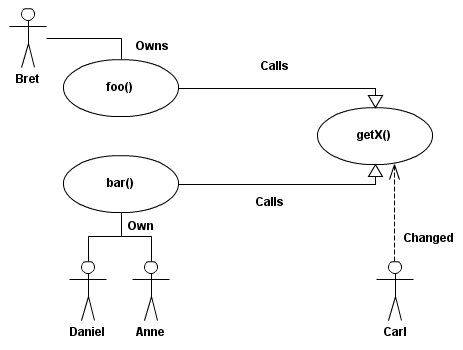
\includegraphics[width=\columnwidth]{images/CallGraph}
\caption{Technical object directed graph with ownership\label{fig:graph}}
\end{figure}

While technical object relationships form the basis of indirect conflicts,
communication between developers is our ultimate goal of resolving such conflicts.
This being the case, developer ownership must be placed on the 
identified technical objects. With this ownership, we now infer
relationships among developers based on their technical objects
``uses'' relationship. Developer A, who owns object 1, which uses 
object 2 owned by developer B, may be notified by a change to
object 2's internal workings. Most, if not all, ownership information
of technical objects can be extracted from a project's source code
repository (CVS, Git, SVN, etc.).

Finally, the indirect conflict tool must be able to detect changes
to the technical objects defined above and notify the appropriate owners
to the conflict. 
Two approaches have been 
proposed for change gathering techniques: real time and commit 
time~\cite{Fitzpatrick:2002:SPA}.
We propose the use of commit time
information gathering as it avoids the issue of developers 
overwriting previous work or deleting modifications which would 
produce information for changes that no longer exist. However, the
trade off is that indirect conflicts must be committed before detected,
which results in conflicts being apart of the system before being able
to be dealt with as opposed to catching conflicts before they happen.
At commit time, the tool must parse changed source code in relation
to technical artifacts in the created directed graph detailed above.
Where \textit{Impact's} design differs from that of Palantir's is that
the object's entire body (method definition and internal body) is 
parsed, similar to that of CASI~\cite{Servant:2010:CPI},
at commit time, as opposed to real time, to detect changes anywhere in the technical object.
This is a first design step towards avoiding information overload.
Once technical objects are found to be changed, appropriate owners
of objects which use the changed object should be notified. However, to
avoid information overload at this step, analyses of the changed object
must be preformed to determine whether or not it is a ``notification worthy''
change. Our proposed solution to this is explained in Section~\ref{sec:ns}.
In Figure~\ref{fig:graph}, Carl changes method (technical object) 1,
which effects methods 2 and 3 resulting in the alerting of
developers Bret, Daniel, and Anne. We have opted to alert the invoking
developers rather than the developer making the change to potential
solutions as our conflicts are detected at commit time and this supports
the idea of a socio-technical congruence~\cite{Kwan:2011:ESC} 
from software structure to communication patterns in awareness systems.

With this three step design: (i) creating directed graphs of technical
objects, (ii) assigning ownership to those technical objects, and (iii)
detecting ``notification worthy'' changes at commit time and the dissemination of conflict information
to appropriate owners, we believe a wide variety of
indirect conflict awareness tools can be created or extended. The
on going implementation of \textit{Impact} described in the following 
section follows these three design guidelines.

\subsection{Implementation}
For \textit{Impact's} implementation, we decided to focus on methods as our
selected technical objects to infer a directed graph from. The ``uses'' 
relationship described above for methods is method invocation.
Thus, in our constructed dependency graph, methods represent nodes
and method invocations represent our directed edges. In order to 
construct this directed graph, abstract syntax trees (ASTs) are 
constructed from source files in the project.

Once the directed graph is constructed, we must now assign
ownership to our technical objects (methods) as per our design.
To do this, we simply query the source code repository. In our case
we used Git as the source code repository, so the command \textit{git blame}
is used for querying ownership information. (Most source code 
repositories have similar commands and functionality.) This command 
returns the source code authors per line which can be used to assign
ownership to methods.

To detect changes to our technical objects (methods), we simply 
use a commit's \textit{diff} which is a representation of all changes
made inside a commit. We can use the lines changed in the \textit{diff} to 
find methods that have been changed. This gives cause of potential
indirect conflicts. Here is where information overload can occur and must
be dealt with. Impact's current state does not address this as our potential 
solution is still under investigation, but is the
main focus of our next steps as detailed in Section~\ref{sec:ns}.
We now find all methods in our directed graphs which invoke these changed methods. 
These are the final indirect conflicts.

Once the indirect conflicts have been found, we use the
ownership information of our technical objects to send notifications to
those developers involved in the indirect conflict. All owners
of methods which invoke those that have been changed are alerted
to the newly changed method. Impact can been seen in
Figure~\ref{fig:impact}, the user interface of \textit{Impact}. Here, in an RSS type
feed, the changing developer, time of change, changed method,
invoking methods, and commit message are all displayed. 
The weight provided will be an indication of importance based
on the future work to be outline in Section~\ref{sec:ns}. This
again helps solve the issue of information overload.

\begin{figure}[t!]
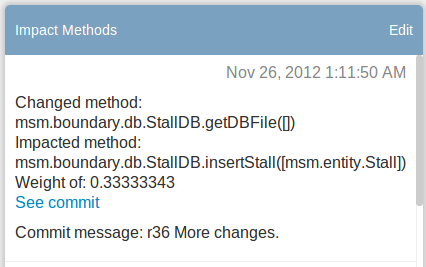
\includegraphics[width=\columnwidth]{images/ImpactDemo}
\caption{\textit{Impact's} RSS type information feed.\label{fig:impact}}
\end{figure}

\section{Proposed Solution to Information Overload}
\label{sec:ns}
As was previously stated, the main issue to be addressed with Impact is
information overload. Our potential solution comes from the ideas of
Meyer~\cite{Meyer:1988} on ``design by contract''. In this methodology, changes to method
preconditions and postconditions are considered to be the most harmful. 
This includes adding conditions that must be met by both input
and output parameters such as limitations to input and expected
output. To achieve this level of source code analysis, the ideas of
Fluri et al.~\cite{Fluri:2007:CDT} can be used on the previously generated
ASTs for high granularity
source code change extraction when determining if preconditions or
postconditions have changed.
We plan to bring these ideas into the realm of what makes a
change ``notification worthy'', as to deal with information overload for
developers using Impact. By only examining ``notification worthy'' changes,
Impact would cut down the number of notifications 
issued to just those which developers care about. To investigate this solution, we plan to
interview and survey industry software developers at a wide range of
experience to determine what makes a change in software important. We believe
by only monitoring what developers and Meyer~\cite{Meyer:1988} find important to
indirect conflict awareness, we will be able to eliminate information overload
in Impact and other dependency awareness tools. We believe that these preconditions
and postconditions will serve as the main tool for dealing with information overload.

\section{Conclusion and Future Work}
In this paper, we have presented the issues that arise from indirect 
conflicts in present awareness tools. We have proposed a generic 
design for the future development of awareness tools in regards to
handling indirect conflicts. We have presented a prototype 
awareness tool, \textit{Impact}, which was designed around our generic 
technical object approach. We have also proposed a solution to information
overload which occurs in most indirect conflict awareness tools. We plan
on investigating our solution further through developer interview and
surveys, and by finally implementing the solution into Impact.


\bibliographystyle{IEEEtran}
\bibliography{paper}

%End of paper
\end{document}